\section[Desenvolvimento do Projeto]{Desenvolvimento do Projeto}

\subsection{Repositório do Código Fonte do Projeto}
  Os repositórios foram divididos entre front-end e back-end, em ambos foi
determinado um padrão de commit estruturado da seguinte maneira, tipo(id user
story): descrição, sendo que a mensagem pode conter no máximo 75 caracteres
para incentivar resumos. O padrão adotado, segue o do Conventional Commits que
busca padronizar e manter relevantes como histórico os commits de um repositório.
Já as branches seguem um padrão inspirado no GitFlow, aprendido na aula
de Gerenciamento e Configuração de Software, estruturados ao redor das branches
main e develop, com cada branch nova seguindo a estrutura tipo/id-task/nome,
garantindo melhor organização na parte do versionamento.
Além disso é notório o uso de Linters, para forçar que a equipe siga estes
padrões, tanto na parte das branches quanto dos commits.

Back-end: \href{https://tools.ages.pucrs.br/industria-digital/industria-digital-backend}{industria-digital-backend}

Front-end: \href{https://tools.ages.pucrs.br/industria-digital/industria-digital-frontend}{industria-digital-frontend}

\clearpage
\subsection{Banco de Dados Utilizado}
  Por uma soma de fatores, como indicação dos stakeholders e
convencionalidade de iniciar o projeto a partir de um banco de dados relacional já
existente da receita, o time optou de primeira mão por continuar no caminho dos
bancos de dados relacionais.

Dentre eles o PostgreSQL foi a nossa escolha, sendo influenciada por fatores
como, domínio do mercado, facilidade de escrita e similaridade com as sintaxes
aprendidas nas matérias de Banco de Dados. Além disso a robustez e capacidade
de lidar com volumes imensos de dados, são características essenciais para nosso
projeto, disponibilizadas pelo PostgreSQL.

  \begin{figure}[H]
    \centering
    \small
    \caption{Modelagem do Banco de Dados - Industria Digital}
    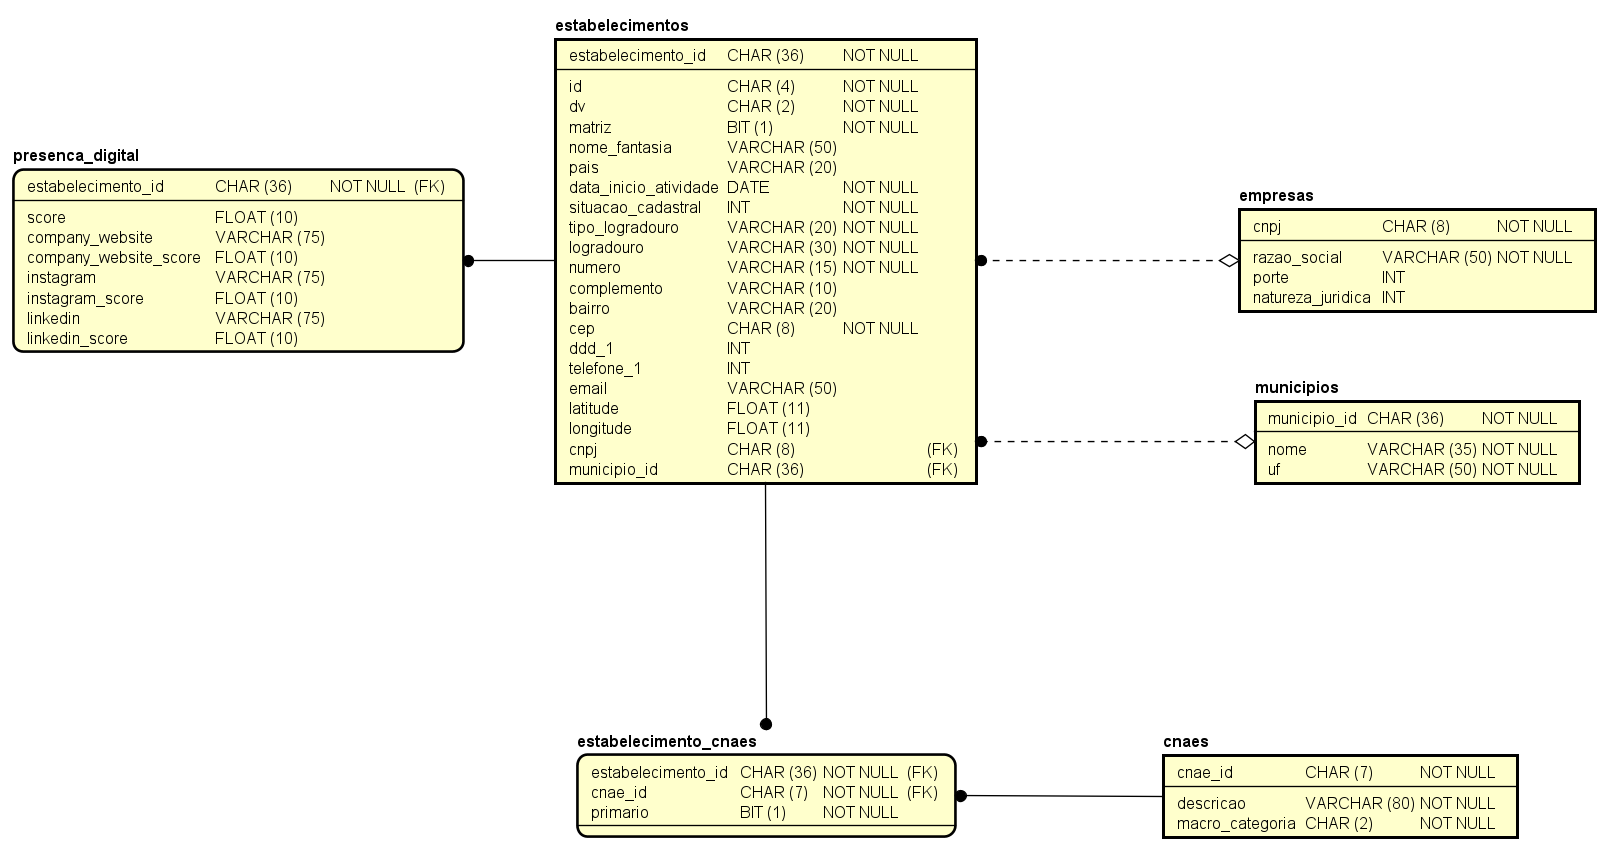
\includegraphics[width=1\linewidth]{conteudo//3 - ages II//conteudo//figures/industria-digital-database.png}
    Fonte: Wiki do Projeto
    \label{fig:database-industria-digital}
\end{figure}

  Como o trabalho tinha o intuito de ser uma prova de conceito, fizemos grande
parte com apenas parcela do banco de dados da receita, portanto foi fundamental
que a equipe deixasse salvo todo script rodado que modifica o banco de dados, já
que eles precisavam ser rodados novamente a cada troca de banco. Exemplos de
modificações que viraram scripts são, conversões de tipo, como cnpj e id que foram
passados de número para string, criação de campos novos, como uma chave
primária estabelecimento\_id, para substituir a chave composta que antes era
utilizada e remoção de campos irrelevantes para o projeto, como fax e ente
federativo responsável, para deixar o banco mais leve. Além disso colocamos uf
como um atributo da tabela municípios para facilitar a busca.

Além disso para conversa do back-end com o banco de dados, estamos
utilizando o ORM, SQLAlchemy, responsável por facilitar a comunicação entre os
dois.

\href{https://tools.ages.pucrs.br/industria-digital/wiki/-/wikis/Banco\%20de\%20dados}{Banco de dados}

\clearpage
\subsection{Arquitetura Utilizada}
  Deverão ser apresentados os links da Wiki, com uma breve descrição.

\clearpage
\subsection{Protótipos das Telas Desenvolvidas}
  Deverão ser apresentados os links da Wiki, com uma breve descrição.

\clearpage
\subsection{Tecnologias Utilizadas}
  Deverão ser apresentados os links da Wiki, com uma breve descrição.
  
  As tecnologias citadas deverão ter referências bibliográficas.
